% .:: Laden der LaTeX4EI Formelsammlungsvorlage
\documentclass[fs, footer]{latex4ei}

% Dokumentbeginn
% ======================================================================
\begin{document}


% Aufteilung in Spalten
\vspace{-4mm}
\begin{multicols*}{4}
	\fstitle{Schaltungstechnik 1}
	
% -------------------------------------------
% | 		Schaltungstechnik				|
% ~~~~~~~~~~~~~~~~~~~~~~~~~~~~~~~~~~~~~~~~~~~
% SECTION ====================================================================================
\section{Mathematische Grundlagen}
% ============================================================================================

\sectionbox{
\subsection{Sinus, Cosinus \quad $\sin^2(x) \bs + \cos^2(x) = 1$}
\setlength{\tabcolsep}{4pt}
\tablebox{
\begin{tabular*}{\columnwidth}{@{\extracolsep\fill}c|c|c|c|c||c|c|c|c@{}} \ctrule
$x$ & $0$ & $\pi / 6$ & $\pi / 4$ & $\pi / 3$ & $\frac{1}{2}\pi$ & $\pi$ & $1\frac{1}{2}\pi$ & $2 \pi$ \\
$\scriptstyle{ \varphi }$ & $\scriptstyle{0^\circ}$ & $\scriptstyle{30^\circ}$ & $\scriptstyle{45^\circ}$ & $\scriptstyle{60^\circ}$ & $\scriptstyle{90^\circ}$ & $\scriptstyle{180^\circ}$ & $\scriptstyle{270^\circ}$ & $\scriptstyle{360^\circ}$ \\ \cmrule
$\sin$ & $0$ & $\frac{1}{2}$ & $\frac{1}{\sqrt{2}}$ & $\frac{\sqrt 3}{2}$ & $1$ & $0$ & $-1$ & $0$ \\
$\cos$ & $1$ & $\frac{\sqrt 3}{2}$ & $\frac{1}{\sqrt 2}$ & $\frac{1}{2}$ & $0$ & $-1$ & $0$ & $1$ \\     
$\tan$ & $0$ & $\frac{\sqrt{3}}{3}$ &	$1$	&	$\sqrt{3}$ & $\pm \infty$ & $0$ & $\mp \infty$ & $0$\\ \cbrule
\end{tabular*} }
}


% SECTION ====================================================================================
\section{Netzwerktheorie}
% ============================================================================================

\sectionbox{

\subsection{Kirchhoff-Gesetze}
Konzentriertheitshypothese: $d << \lambda$ mit \\
$d = $ Größe der Schaltung, Wellenlänge $\lambda = c T$ \\

Knotenregel \emph{KCL}: $ \sum \limits_{\text{Knoten}}i_{\ir j} (t) = 0$ (heraußfließende Ströme positiv) \\
Maschenregel \emph{KVL}: $ \sum \limits_{\text{Umlauf}} u_{\ir j} (t) = 0$ (Spannungen in Umlaufrichtung positiv)

Knoteninzidenzmatrix: $\ma A' = \mat{\alpha_{11} &  \ldots & \alpha_{1b} \\ \vdots & &  \\ \alpha_{n1} & \ldots & \alpha_{nb}}$ $n$ Knoten

Spaltensummen von $A'$ sind immer $= 0$ \\
$\Ra$ Zeile des Bezugsknotens streichen $\Ra$ \\
$\ma A \vec i =0$ (reduzierte Knoteninzidenzmatrix)

$\ma M = \ma A^{'\top} $ mit $\vec u = \ma M^{'} \vec u^{'}_{\ir k}$ $\Ra $ KVL in Matrixform: $\vec u - \ma A^{\top} \vec u_{k} = 0$

}



\sectionbox{	
	\subsection{Schaltung und Netzwerkgraph}
	% Verbindet man mehrere Bauelemente zu einer Schaltung ergibt sich eine eindeutige Verbindungsstruktur.\\
	Der gerichtete Netzwerkgraph stellt die Verbindungsstruktur einer Schaltung durch $n$ Knoten (node) und $b$ Verbindungskanten (branch) mit Richtungspfeilen dar.\\
	Jedes Bauelement mit zwei Anschlüssen entspricht einer Verbindungskante. Ein Knoten ist dort, wo ein oder mehr Anschlüsse von Bauteilen durch ideal leitenden Draht miteinander verbunden sind.
	Verbundene Anschlüsse entsprechen einem Kurzschluss, nicht verbundene Anschlüsse einem Leerlauf!


	Um die Betriebspunkte einer Schaltung zu bestimmen sind $2b$ linear unabhängige Gleichungen nötig. Man erhält diese $2b$ Gleichungen aus den Beschreibungen der Bauelemente und den Kirchoff Gleichungen.


	\subsubsection{Wichtige Begriffe}
		\begin{description}%\itemsep0pt
		\item[Zählpfeile:] Zeigen die gemeinsame(assoziierte) Zählrichtung von Stromfluss und Spannungsabfall zwischen zwei Knoten an, unabhängig von den tatsächlichen Richtungen(Vorzeichen).
		\item[Masse(Erdung) $\perp$:] Bezugspunkt des elektr. Potentials mit Potential $0V$
		\item[Kurzschluss(KS):] ideal leitender Draht. $u_{KS} = 0$, $i_{KS}=$beliebig
		\item[Leerlauf(LL):] ideal isolierende Luft. $u_{LL}=$beliebig, $i_{LL} = 0$
		\item[Tor:] Ein Tor bilden zwei Anschlüsse bei denen der Stromzufluss des einen Anschluss gleich dem Stromabfluss des anderen Anschluss entspricht. $i_{in} = i_{out}$
	\end{description}	

}

	\subsection{Eintorverschaltungen}


	\tablebox{
	\begin{tabular*}{\columnwidth}{@{\extracolsep\fill}ll@{\hspace{1em}}|ll@{}} \ctrule
		\multicolumn{2}{c}{\large{Serienschaltung}} & \multicolumn{2}{c}{\large{Parallelschaltung}} \\ \ctrule
		$u= \sum u_i$ & $i=\const$ & $u =\const$ & $i=\sum i_i$\\
		$q= \const$ & $\Phi_{\ir M} =\sum \Phi_{{\ir M,}i}$  & $q=\sum q_i$ & $\Phi_{\ir M}=\const$\\ \cmrule
		$R=\sum R_i$ & $M=\sum M_i$ & $\frac{1}{R} = \sum \frac{1}{R_i}$ & $\frac{1}{M} = \sum \frac{1}{M_i}$\\[0.5em]
		$\frac{1}{C} = \sum \frac{1}{C_i}$ & $L=\sum L_i$ & $C=\sum C_i$ & $\frac{1}{L} = \sum \frac{1}{L_i}$ \\[0.5em] \cmrule
		$\cx Z=\sum \cx Z_i$ & $\frac{1}{\cx Y} = \sum \frac{1}{\cx Y_i}$ & $\frac{1}{\cx Z} = \sum \frac{1}{\cx Z_i}$ & $\cx Y=\sum \cx Y_i$\\ \cbrule
	\end{tabular*} }



\sectionbox{
\subsection{Resistive Eintore}

\begin{itemize}
	\item Implizite Darstellung: $f_F (u,i) = 0$
	\item Parameterdarstellung: $u = u_F ( \lambda )$ \quad $ i = i_F (\lambda )$ 
	\item Explizite Darstellung: $\underset{\ir Leitwertdarstellung}{i = g_F (u)}$ \quad $\underset{\ir Widerstandsdarstellung}{u = r_F (i)}$
	\item Umpolung: $\overline F$ entsteht durch Punktspiegelung von $F$ am Unsprung: $(\overline u, \overline i) = (- u, - i) \in \overline F$
	\item Dualität: $(u,i) \in F \Leftrightarrow ( R_d i, \frac{ u}{ R_d}) \in F^d$
	\item Parallelschaltung von Widerstandsgeraden: $G = G_1 + G_2$ \\
	$\Ra \frac 1 R = \frac 1 R_1 + \frac 1 R_2 \Ra R = R_1 \parallel R_2 = \frac{R_1 R_2}{R_1 + R_2}$
	\item Serienschaltung von Widerstandsgeraden: genauso wie Parallelschaltung nur $R$ statt $G$
	\item Arbeitspunkt ermitteln:
		\begin{enumerate}
			\item Schaltungs aufteilen in Quelle $Q$ und Last $L$
			\item Parameterdarstellung $\Ra$ Kennlinien zeichnen
			\item Lösung: Schnittpunkte der Kennlinien! $\Ra$ ist die Funktion im AP stetig und diffbar, kann man sie dort \emph{linearisieren}
		\end{enumerate}
\end{itemize} 

Eigenschaften von $F$:

\tablebox{
	\begin{tabular*}{\columnwidth}{@{\extracolsep\fill}ll@{}}
	\ctrule
		F ungepolt & Kennlinie punktsymm. zum Ursprung \\ 
		F aktiv & mind. 1 Pkt. in II. od. IV. Quadr. \\
		F verlustfrei & nur auf Koordinatenachsen \\
		F quellenfrei & enthält den Ursprung \\
		F streng linear & $(ku, ki) \in F$ \quad $ (u_1 + u_2, i_1 + i_2) \in F$ \\
		\cbrule
	\end{tabular*}
}


}
% -- Seite 1



\newpage
% -------------------------------------------------------
% | 		S C H A L T U N G S T E C H N I K 2			|
% ~~~~~~~~~~~~~~~~~~~~~~~~~~~~~~~~~~~~~~~~~~~~~~~~~~~~~~~
%########################################################################################################################################################################################################
{\huge{\textbf{Schaltungstechnik 2}}} 


\section{Allgemeines}
% ===============================================================================================
	
	\subsection{Die vier zentralen Größen $u,i,q,\Phi$}
	% ----------------------------------------------------------------------
	... beschreiben die Wirkungsweise von elektronischen Bauelementen.\\ \\
	\begin{tabular}{lc|ll}
		Größe & & Definition\\ \hline
		Spannung & $u$ & Potentialdifferenz. Richtung: Von hohem zu niedrigen Potential.\\
		Stromfluss & $i$ & Bewegte Ladung. Richtung: Bewegungsrichtung positiver Ladung.\\
		Ladung & $q$ & Grundeigenschaft von Materie. Es gibt positive und negative Ladung.\\
		Magn. Fluss & $\Phi$ & Grundeigenschaften von elektr. magn. Feldern.\\
	\end{tabular} 
	
		\subsubsection{Allgemeine Zusammenhänge $u,i,q,\Phi$}
		Ladung und Strom beschreiben den Zustand der Materie.\\
		Spannung und magn. Fluss beschreiben den Zustand des elekt. magn. Feldes.\\ \\
		\begin{tabular}{l|l}
			$i(t) = \dot q(t)$ & $[i]=A$\\
			$q(t) = q(t_0) + \int_{t_0}^t i(\tau) \mathrm d\tau$	& $[q]=As=C$ \\ \hline
			$u(t) = \dot \Phi(t)$ & $[u]=V$\\
			$\Phi = \Phi(t_0) + \int_{t_0}^t u(\tau) \mathrm d\tau$ & $[\Phi]=Vs=Wb$ \\
		\end{tabular}
	



		\subsubsection{Arten von Bauelementen}
		\begin{tabular}{l|l|l|l|l}
			Art & Symbol & Beschr. & linear & Beispiel\\ \hline
			Resistivität & 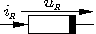
\includegraphics[height=0.4cm]{./img/Resistivitat.pdf} & $f_R(u,i)$  & $u = U_0 + R \cdot i$ & PN-Diode\\
			Kapazität & 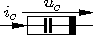
\includegraphics[height=0.4cm]{./img/Kapazivitat.pdf} & $f_C(u,q)$ & $q = Q_0 + C \cdot u$ & Kondensator\\ 
			Induktivität & 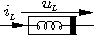
\includegraphics[height=0.4cm]{./img/Induktivitat.pdf} & $f_L(i,\Phi)$ & $\Phi = \Phi_0 + L \cdot i$ & Spule\\
			Memristivität & 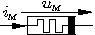
\includegraphics[height=0.4cm]{./img/Memristivitat.pdf} & $f_M(q,\Phi)$ & $\Phi = \Phi_0 + M \cdot q$ & Memristor\\
		\end{tabular}





\sectionbox{	
	\subsection{Komplexe Wechselstromrechnung}
	% ---------------------------------------------------------
	Vorraussetzung: lineares, eingeschwungenes System mit sinusförmiger Erregung $x(t) = \hat x \cdot \cos(\omega t + \varphi)$
	Effektivwert $X = \frac{\hat x}{\sqrt{2}}$\\
	Differentialoperator: $\frac{\diff}{\diff t} = \i \omega$\\
	\emphbox{
	\begin{tabular}{ll}	
		Reeles Zeitsignal: &\!\!\!\!\!\! $x(t) = \hat x \cdot \cos(\omega t + \varphi_x)$\\[0.5em]
		Effektiver Zeiger: &\!\!\!\!\!\! $\cx X = X_w + \i X_b = X \exp(\i \varphi_x)$\\[0.5em]
		Scheitel Zeiger: &\!\!\!\!\!\! $\boldsymbol{\hat X} = \sqrt{2} \cx X = \hat X \exp(\i \varphi_x)$\\[0.5em]
		Kompl. Zeitsignal: &\!\!\!\!\!\! $\cx x(t) = \boldsymbol{\hat X} \cdot e^{\i \omega t} = \hat x \cdot e^{\i(\omega t + \varphi_x)}$\\[0.5em]
		Phase: &\!\!\!\!\!\! $\varphi_x := \arg \cx X = \arctan \frac{X_b}{X_w}$\\
	\end{tabular} }	\\
	\framebox[\columnwidth]{
		\begin{tabular}{l@{\hspace{4em}}l}
		$\underset{\text{Impedanz}}{\cx Z(j\omega)} = \underset{\text{Resistanz}}{R(j\omega)} + \underset{\text{Reaktanz}}{jX(j\omega)}$ & $\cx U = \cx Z \cdot \cx I$\\[0.5em]
		$\underset{\text{Admittanz}}{\cx Y(j\omega)} = \underset{\text{Konduktanz}}{G(j\omega)} + \underset{\text{Suszeptanz}}{jB(j\omega)}$ & $\cx I = \cx Y \cdot \cx U$\\
		\end{tabular}
	}

	\tablebox{
	\begin{tabular*}{\columnwidth}{l@{\extracolsep\fill}cccc} \ctrule
	 & \textbf{Widerstand} & \textbf{Kondensator} & \textbf{Spule} & \textbf{Memristor}\\ \cmrule
	$Z=$ & $R$ & $\frac{1}{j \omega C}$ & $j \omega L$ & $M$\\[0.5em]
	$Y=$ & $G = \frac{1}{R}$ & $j \omega C$ & $\frac{1}{j \omega L}$ & $\frac{1}{M}$\\[0.5em]
	$\underset{\varphi_u - \varphi_i}{\Delta \varphi =}$ & 0 & $-\frac{\pi}{2}$ & $\frac{\pi}{2}$ & ?\\ \cbrule
	\end{tabular*} }
}







% Ende der Spalten
\end{multicols*}

% Dokumentende
% ======================================================================
\end{document}

% ToDos:

